\documentclass[12pt]{report}

%  ********** Incluir packages **********
\usepackage[english,spanish]{babel} % Out: Idiomas usados
\usepackage{lmodern}           % Out: Fuente "Latin Modern"
\usepackage[T1]{fontenc}       % Out: Encoding de la fuente
\usepackage[utf8]{inputenc}    % In:  Encoding de los archivos de entrada
\usepackage{graphicx}          % Importar imágenes y gráficos
\usepackage{datetime}          % Acceso a variables de fecha
\usepackage{fancyhdr}          % Cabecera de página (numeración)
\usepackage{titlesec}          % Cambiar formato de título en los capitulos y otros.
\usepackage[table]{xcolor}     % Colores
\usepackage{dcolumn}           % Columnas alineadas por punto decimal
%\usepackage{listings}          % Código fuente
%\usepackage{array}             %
\usepackage{caption}           % Soporte para subfiguras
\usepackage{subcaption}        % Soporte para subfiguras
\usepackage{amsfonts}          %
\usepackage{mathtools}         %
\usepackage[hyperref=true]{acro} % Acrónimos
\usepackage[bookmarks=true,bookmarksnumbered, colorlinks=t, hidelinks, breaklinks]{hyperref}
% Margenes y tamaño de la página
\usepackage[letterpaper, top=2.5cm, bottom=2cm, left=2.5cm, right=2cm, headsep=0.3cm]{geometry}

%  ********** Definir autor, prof. patrocinante, título y fecha de la memoria **********
\newcommand{\AuthorName}{Aldo Nicolás Mellado Opazo}
\newcommand{\AdvisorNameA}{Dr. Sergio Sobarzo Guzmán.}
\newcommand{\MainTitle}{Sistema de posicionamiento indoor mediante seguimiento de direcciones MAC de equipos móviles}
\newcommand{\Career}{Ingeniería Civil en Telecomunicaciones}
\newcommand{\CTitle}{Ingeniero Civil en Telecomunicaciones}
%\newcommand{\MyCustomDate}{Julio de 2015} % Comentar para poner fecha automáticamente

%  ********** Configurar packages y otras cosas **********
% -- Bibliography style (BibTeX) --
\bibliographystyle{IEEEtran}
% -- graphicx --
\graphicspath{{./images/}}
%
% -- fancyhdr (numaración de páginas) --
\fancypagestyle{plain}{%
\fancyhf{}
\fancyhead[R]{\thepage}
\renewcommand{\headrulewidth}{0pt}
\renewcommand{\footrulewidth}{0pt}
}
%
% -- titlesec (estilo de título) --
\titleformat{\chapter}[hang]{\bfseries\huge}{\thechapter.}{2ex}{}
\titlespacing{\chapter}{0cm}{0cm}{0cm}
%
% -- caption y subcaption --
\captionsetup[figure]{skip=2pt}
\captionsetup[subfigure]{skip=0pt}
\captionsetup[table]{skip=2pt}
% -- acro: Acrónimos --
% Para arónimos en inglés
\newcommand{\MyCustomListStyle}[1]{(del inglés \itshape{#1})}
\acsetup{ foreign-format = {del inglés \itshape} }
\acsetup{ list-foreign-format = {\MyCustomListStyle} }

% ********** Interlineado, salto de párrafo y sangría **********
% Para interlineado de 1.5 poner: 1.3
% Para interlineado de 2.0 poner: 1.6
\linespread{1.3}
%\setlength{\parindent}{1cm}
\setlength{\parskip}{0.4cm}


% Archivo con definición de acrónimos

% Template: \DeclareAcronym{} { short = , long = , foreign = }
\DeclareAcronym{ASIC}  { short = ASIC, long = circuito integrado de aplicación específica, foreign = Application-Specific Integrated Circuit}
\DeclareAcronym{CMOS}  { short = CMOS, long = semiconductor complementario de óxido metálico, foreign = Complementary Metal Oxide Semiconductor}
\DeclareAcronym{FPGA}  { short = FPGA, long = arreglo de compuertas programables, foreign = Field Programmable Gate Array}
\DeclareAcronym{NAVSAT}{short= NAVSAT, long= Sistema Satelital de Navegación Naval, foreign= Navy Navigation Satellite System}
\DeclareAcronym{GPS}{short = GPS,long = Sistema de Posicionamiento Global, foreign = Global Positioning System}
\DeclareAcronym{AP}{short = AP,long  = Punto de Acceso, foreign= Access Point}
\DeclareAcronym{MAC}{short= MAC,long = Control de Acceso al Medio, foreign =Media Access Control}
\DeclareAcronym{RNN}{short= RNN,long = Red Neuronal Recurrente, foreign = Recurrent Neural Network}
\DeclareAcronym{IPS}{short = IPS,long  = Sistema de Posicionamiento en Interiores, foreign= Indoor Positioning System}
\DeclareAcronym{RSSI}{short= RSSI, long = Indicador de Intensidad de Señal Recibida, foreign = Received Signal Strengh Indicator}
\DeclareAcronym{AoA}{short= AoA,long= Ángulo de llegada ,foreign = Angle of Arrival}
\DeclareAcronym{ToA}{short= ToA,long= Tiempo de llegada ,foreign = Time of Arrival}
\DeclareAcronym{ToF}{short= ToF,long = Tiempo de Vuelo ,foreign = Time of Flight}
\DeclareAcronym{KNN}{short= KNN ,long = K-Vecinos más Cercanos, foreign= K-Nearest Neighbour}
\DeclareAcronym{RSS}{short = RSS, long= Nivel de Intensidad de Señal Recibida, foreign = Received Signal Strenght}
\DeclareAcronym{TDoA}{short = TDoA, long = Diferencia de Tiempo de Llegada, foreign = Time Difference of Arrival}
\DeclareAcronym{RToF}{short=  RToF, long= Ruta de Viaje de Vuelo, foreign = Round-Trip Time of Flight}
\DeclareAcronym{NLOS}{short = NLOS, long = No Línea de Vista, foreign = None Line of Sight}
\DeclareAcronym{RN}{short = RN, long = Redes Neuronales, foreign = Artificial Neural Network}
\DeclareAcronym{RN  N}{short = RNN, long = Red Neuronal Recurrente, foreign = Recurrent Neural Network}
\DeclareAcronym{KWNN}{short=KWNN, long= K-Vecino Ponderado Más Cercano,foreign = K-Weighted nearest neighbor}
\DeclareAcronym{SVM}{short = SVP,long = Máquinas de vectores de soporte,foreign = Support Vector Machine }
\DeclareAcronym{SMP}{short = SMP,long = Polígono más pequeño de M-Vértices ,foreign = Smallest M-Vertex Polygon}
\DeclareAcronym{LOS}{short = LOS,long = Línea de Vista, foreign = Line of Sight}
\DeclareAcronym{FCC}{short = FCC, long = Comisión Federal de Comunicaciones, foreign = Federal Communications Commission}
\DeclareAcronym{RTT}{short=RTT,long = Tiempo-de-Viaje, foreign = Round-Trip-Time}
\DeclareAcronym{BLE}{short=BLE, long = Bluetooth de Baja Energía, foreign = Bluetooth Low Energy}
\DeclareAcronym{UWB}{short = UWB, long = Banda Ultra Ancha, foreign = Ultra Wide-Band}

\begin{document}
% ******************** Algunas definiciones ********************
\renewcommand{\contentsname}{Índice General}
\renewcommand{\listfigurename}{Índice de Figuras}
\renewcommand{\listtablename}{Índice de Tablas}
\renewcommand{\figurename}{\textbf{Fig.}}
\renewcommand{\tablename}{\textbf{Tabla}}


% ******************** Portada ********************
	% Hoja 1
	\pdfbookmark{Portada}{portada}
	\thispagestyle{empty}
	\begin{titlepage}
\begingroup

% Esta página usa interlineado simple sin saltos de párrafo
\linespread{1}\selectfont
\setlength{\parskip}{0pt}
	
{ \vspace*{2 pc} }

\begin{center}
	\textbf{\LARGE UNIVERSIDAD DE CONCEPCIÓN} \\[0.4 pc]
	{\large FACULTAD DE INGENIERÍA} \\[0.4 pc]
	{ DEPARTAMENTO DE INGENIERÍA ELÉCTRICA} \\[0.4 pc]
\end{center}

\vspace{6 pc}

\noindent\begin{minipage}{0.35\textwidth}\hfill\end{minipage}
%
\begin{minipage}[t]{0.25\textwidth}
	\centering
	
\includegraphics[width=3.2cm]{logos/logo_udec}
\end{minipage}
%
\hspace*{0.5cm}
%
\begin{minipage}{0.34\textwidth}
	Profesor Patrocinante: \\[0.4 pc] \textbf{\AdvisorNameA} \\
	\vskip 4.3cm
	Informe de Memoria de Título \\
	para optar al título de: \\[0.4 pc]
	\textbf{Ingeniero Civil en Telecomunicaciones}
\end{minipage}

\vspace{9 pc}

\begin{center}
	\textbf{\LARGE \MainTitle}
\end{center}
%
%
\vfill
Concepción,
\ifdefined\MyCustomDate
	\MyCustomDate
\else
	{\monthname} de \the\year
\fi
\hfill \AuthorName
%
%
\endgroup
\end{titlepage}


	% Hoja 2
	\thispagestyle{empty}
	\begin{titlepage}
\begingroup

% Esta página usa interlineado simple sin saltos de párrafo
\linespread{1}\selectfont
\setlength{\parskip}{0pt}

% Universidad y supervisor
\begin{minipage}{0.45\textwidth}
	Universidad de Concepción \\ Facultad de Ingeniería \\ Departamento de Ingeniería Eléctrica
\end{minipage}
%
\hfill
%
\begin{minipage}{0.45\textwidth}
	\raggedleft
	Profesor Patrocinante: \\ \AdvisorNameA 
\end{minipage}
%
%
\begin{center} 
	\vspace{5cm}
	
	\textsc{\huge \MainTitle}\\[5.5cm]

	{\large \AuthorName}\\[1.5cm]

	Informe de Memoria de Título\\
	para optar al Título de\\[1.5cm] 

	\CTitle
	\vfill

	% Final de la página
	\ifdefined\MyCustomDate
		{\large \MyCustomDate}
	\else
		{\large {\monthname} \the\year}
	\fi
\end{center}

\endgroup
\end{titlepage}



% ******************** Resumen y agradecimientos ********************
	% Numeración: Romana, i.e. I, II, III, etc.
	% página no numerada
	\newpage
	\pagestyle{plain}
	\pagenumbering{roman}
	\setcounter{secnumdepth}{-1}
%    \chapter{Resumen}

Lorem ipsum dolor sit amet, consectetur adipiscing elit, sed do eiusmod tempor incididunt ut labore et dolore magna aliqua. Ut enim ad minim veniam, quis nostrud exercitation ullamco laboris nisi ut aliquip ex ea commodo consequat. Duis aute irure dolor in reprehenderit in voluptate velit esse cillum dolore eu fugiat nulla pariatur. Excepteur sint occaecat cupidatat non proident, sunt in culpa qui officia deserunt mollit anim id est laborum.

Un \ac{FPGA} se puede usar en las etapas de diseño de un \ac{ASIC}.
Aunque los \acp{FPGA} también tienen otros usos.

\acresetall

    
%    %---------- Primera hoja ----------
\vspace*{\fill}

\begin{flushright}
    {\large A los semiconductores...}\\
    {\large \emph{Gracias por todo}}
\end{flushright}
\vspace*{\fill}


%---------- Segunda hoja ----------
\newpage
\chapter{Agradecimientos}

Lorem ipsum dolor sit amet, consectetur adipiscing elit, sed do eiusmod tempor incididunt ut labore et dolore magna aliqua. Ut enim ad minim veniam, quis nostrud exercitation ullamco laboris nisi ut aliquip ex ea commodo consequat. Duis aute irure dolor in reprehenderit in voluptate velit esse cillum dolore eu fugiat nulla pariatur. Excepteur sint occaecat cupidatat non proident, sunt in culpa qui officia deserunt mollit anim id est laborum.



% ******************** Índice ********************
    \newpage
    \begingroup
    \setlength{\parskip}{0pt}
    % Profundidad de numeración en el índice
    \setcounter{secnumdepth}{3}
    % Profundidad de numeración en el texto
    \setcounter{tocdepth}{3}
    \pdfbookmark{\contentsname}{toc}
    \tableofcontents
	\endgroup


% ******************** Índice de figuras ********************
	\newpage
	\phantomsection
	\addcontentsline{toc}{chapter}{\listfigurename}
	\listoffigures


% ******************** Índice de tablas ********************
    \newpage
    \phantomsection
    \addcontentsline{toc}{chapter}{\listtablename}
    \listoftables


% ******************** Acrónimos ********************
	\newpage
	\printacronyms[name=Siglas]


% ******************** Capítulos ********************
	% Numeración normal, i.e. 1, 2, 3, etc.
    \newpage
    \pagenumbering{arabic}

    
\chapter{Introducción}

\section{Antecedentes históricos}
El ser humano, en la década del 60, ante la incipiente necesidad de saber su posición en el planeta desarrolló un sistema de posicionamiento  llamado OMEGA y posteriormente otro llamado TRANSIT o \ac{NAVSAT}, que  fue resultado del trabajo conjunto de la NASA y el departamento de defensa de los Estados Unidos. Años después este acabó siendo reemplazado debido a la falta de precisión que este tenía, y que alcanzaba un error de hasta 250 metros.

Su sucesor apareció en la década del 70 bajo el nombre de \ac{GPS} y su precisión permitía posicionar un objeto con un error de menos de 5 metros. Esto a través del cálculo del tiempo que tarda en llegar la señal al receptor, es decir, el efecto Doppler.

Funciona actualmente con un mínimo de 24 satélites en órbita sobre la tierra cuyas trayectorias sincronizadas le permiten mapear completamente el planeta y entregar posicionamiento casi exacto a dispositivos móviles y vehículos.

Existen desde ya hace décadas intentos por emular lo logrado con el GPS, pero para espacios interiores, estos intentos han recibido el nombre de \ac{IPS}, que conforme a lo que se presentará en capítulos posteriores han logrado obtener resultados de posición con márgenes de error inferiores a los 3 m. 

\section{Definición del problema}
Las condiciones bajo las cuales es posible para la señal propagarse no se cumplen en todos los ambientes. Existen lugares en que a diferencia de lo que sucede en el exterior, donde la señal se refleja haciendo posible la triangulación de la posición, esta se absorbe parcial o completamente y principalmente corresponden a espacios interiores, tales como una bodega, un centro comercial o una oficina, haciendo que posicionarse dentro de estos espacios sea imposible a través del GPS, es por esto que a fin de brindar nuevas experiencias a usuarios a través del posicionamiento dentro de estos espacios se han desarrollado soluciones utilizando la banda de los 2.4 [GHz] que es la utilizada por, entre otros tecnologías, el Wi-Fi. 

Esta ha sido ampliamente estudiada debido a la alta penetración comercial que ha alcanzado precisamente en estos espacios donde el GPS no da cobertura, sin embargo, dentro de los distintos enfoques en que se han abordado los estudios se tiene que la medición de los niveles de potencia radiada desde los \ac{AP}, a través de los cuales se realiza la triangulación de la posición, se ven altamente afectados por la variación del escenario caracterizado. Este tipo de variaciones pueden ser inducidas por la presencia de personas u objetos que reflejen o absorban la señal.

Es por esto que el método a través del cual se de solución al problema del posicionamiento en interiores debe ser un \ac{IPS} capaz de compensar la incidencia de estas variaciones en el \ac{RSSI} dentro de la operación del algoritmo y así, estimar correctamente la posición de objetivo deseado identificable a través de su dirección de \ac{MAC}.

\section{Estado del arte}

En cuánto a los enfoques que se han considerado para evaluar la posición de un dispositivo móvil en un espacio interior se han podido desarrollar diversas soluciones que apuntan de una u otra manera a aproximaciones geométricas. A fin de ordenar según la técnica, la documentación consultada, se hará una clasificación y dentro de las categorías, explicará las investigaciones en el área.\\

%%%%%%%%%%%%%%%%%%%%%%%%%%%%%%%%%%%%%%%%%%%%%%%%%%%%%%%%%%
                \clearpage 
%%%%%%%%%%%%%%%%%%%%%%%%%%%%%%%%%%%%%%%%%%%%%%%%%%%%%%%%%%

Se abordará siguiendo el esquema que está a continuación:
\begin{figure}[h!]
    \centering
    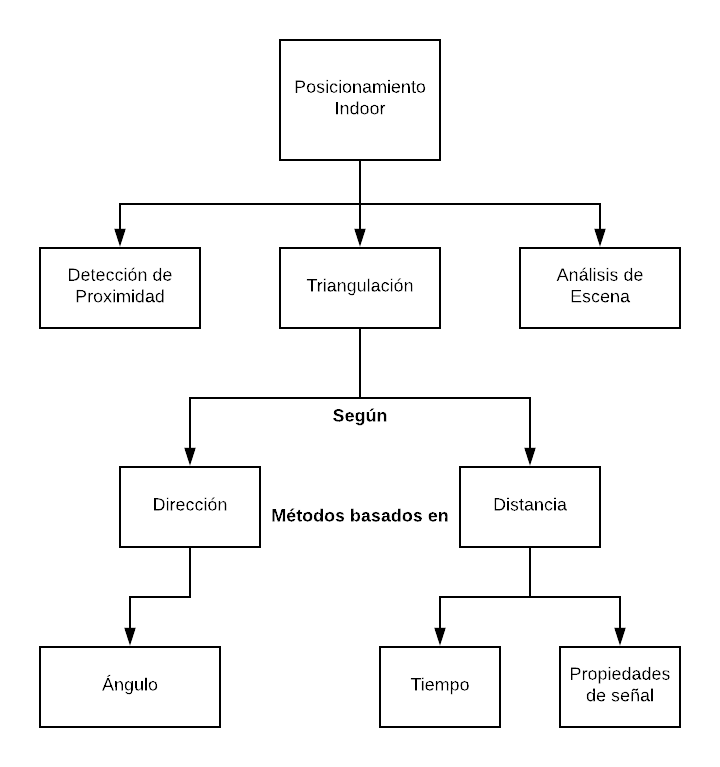
\includegraphics[scale = 0.3]{./images/diagrama}
    \label{fig:diagrama}
\end{figure}

%\begin{itemize}
%\item{\ac{AoA}: Referido, como su nombre lo dice, se refiere al ángulo de llegada de la señal del dispositivo móvil, proveniente de una ubicación desconocida, la cual es recibida en múltiples estaciones base. Resultaría provechoso un sistema de posicionamiento de este tipo puesto que solo requiere dos AP o Beacons, cuya precisión puede ser mejorada por la inclusión de un tercero. \\

%En este caso, y tal y como explican \textit{Kyle Davies e Ian Jones }en \cite{11}, si se incluye un tercer elemento se habla de triangulación:

%\begin{itemize
%\item{\textbf{Triangulación:} Este método, explicado en \textit{Recent Advances in Wireless Indoor Localization Tecniques and System}\cite{6} usa herramientas geométricas de triángulos para determinar la ubicación del objetivo. Tiene a su vez dos posibles variaciones:

% Trilateración: Si es que en lugar de usar propiedades geométricas de triángulos, utiliza círculos que corresponden al área de cobertura del AP. Estos a través de un punto de intersección de las circunferencias permiten estimar la posición del objetivo. Se basa en el nivel de RSS. Esto fue utilizado en \cite{3}, \cite{4}, \cite{5}, \cite{7}, \cite{8} y \cite{9}.}
% \end{itemize}

% En estos papers, específicamente en el trabajo de Zahid, Rosdiadee y Mahamod, ellos recopilaron información detallada sobre las técnicas de posicionamiento indoor a la fecha de publicación, hacen una diferencia respecto cuándo usar Trilateración o Triangulación, mencionando que cuando se trata de técnicas de medición de propagación basadas en tiempo, esto es \ac{ToF}, RTOF y TDOA o en RSS, se puede usar un algoritmo del tipo Trilateración, mientras que si se trata de AoA, el algoritmo a usar es el de Triangulación. 

% Sin embargo, esta aproximación depende del uso de antenas altamente directivas o bien, de arreglos de antenas lo que ciertamente aumenta sustancialmente el costo de su implementación. Ya que lo que se usa son relaciones geométricas que permiten estimar el punto de intersección. }

% \item{\ac{ToF}, este concepto está referido a la técnica a través de la cual se realizan cálculos de posición a través del tiempo de llegada de la señal respecto de diversos puntos de referencia.}
% \end{itemize}

% No obstante, las técnicas más usadas dentro de las consultadas en la revisión bibliográfica son aquellas que usan un método combinado de herramientas matemáticas del tipo estadísticas, en conjunto con los valores de RSS, para estimar la posición. Las herramientas son utilizadas para corregir errores que se producen en la recepción de la señal y que se originan en las reflexiones que esta experimenta a través del viaje desde y hacia el dispositivo.

% Se reconocen además dos fases muy bien definidas en el proceso de desarrollo de un sistema de posicionamiento. Una fase \textit{offline}, que guarda relación con el mapeo o la caracterización del espacio en función de los valores de intensidad de señal recibida en los cuadrantes en que se divide el espacio sobre el cual se moverá el dispositivo, y una fase \textit{online}, que es en la cual el dispositivo movil se mueve a través de este espacio enviando los RSSI a un servidor que consulta en la base de datos obtenida previamente, cuál es o debería ser la posición de este en el espacio.

% Sin embargo, sugieren autores en \cite{8}, \cite{11}, \cite{12} y \cite{14}, que la precisión mejora considerablemente, al rededor de un 45\% sobre los resultados preliminares, si es que se considera la media y la desviación estándar en los resultados.

%%%%%%%%%%%%%%%%%%%%%%%%%%%%%%%%%%%%%%%%%%%%%%%%%%%%%%%%%%
                \clearpage 
%%%%%%%%%%%%%%%%%%%%%%%%%%%%%%%%%%%%%%%%%%%%%%%%%%%%%%%%%%

\section{Hipótesis de trabajo}
\begin{center}
\textit{''Es posible posicionar un dispositivo, identificable a través de su MAC, en un espacio interior utilizando una \ac{NN} para compensar las variaciones de RSS de los \ac{AP} usados en la trilateración''}
\end{center}

\section{Objetivos}
A continuación se señalan los objetivos que apuntan a resolver el problema presentado y a probar la hipótesis de trabajo.

\subsection{Objetivo general}
Posicionar un dispositivo móvil, reconocible a través de su \ac{MAC} dentro de un espacio interior, a través de algoritmos de trilateración y \ac{NN}.

%\section{Objetivos específicos}
%\begin{enumerate}
%\item{a}
%\end{enumerate}

\section{Alcances y limitaciones}
El alcance de este proyecto estará limitado a encontrar la posición de un dispositivo móvil dentro del espacio del segundo piso de Edificio Tecnológico Mecánico de la Universidad de Concepción. Se ejecutará el algoritmo desarrollado en una laptop personal, utilizando Raspberry Pi como \ac{AP} y el resultado del posicionamiento se desplegará en una interfaz gráfica desarrollada en python.

\section{Metodología}

Para lograr posicionar un dispositivo móvil dentro del espacio interior, se buscará en primera instancia extraer los datos de RSSI obtenidos desde las tarjetas de Red de las placas. Posterior a esto se caracterizará el espacio de trabajo con sus respectivos niveles de RSS. Estas serán usadas para entrenar un modelo que, a través de RNN, pueda detectar la posición en que se halla un usuario, respecto de los niveles de potencia y la certidumbre que arroje el entrenamiento realizado. Finalmente, el resultado será desplegado en una interfaz gráfica.

%	\chapter{Marco Teórico}

\section{Aplicaciones y aproximaciones en sistemas de posicionamiento indoor}

En cuánto a los sistemas de posicionamiento indoor, diversas documentaciones revisadas señalan la importancia de desarrollar esta tecnología a fin de resolver necesidades ya reconocidas dentro de espacios interiores tales como hospitales, museos, parques, etc. Sin embargo, todos concuerdan en que la tarea no es sencilla y por este motivo se ha intentado abordar este problema de distintas maneras, teniendo cada una sus respectivas ventajas y limitaciones.

La clasificación de estos métodos pasa por si es que en ellos se utilizan propiedades físicas o bien, reconocimiento de imágenes. De este modo, un posible ordenamiento es el que sigue:

\begin{itemize}
    \item{Análisis de escena}
    \item {Detección de proximidad}
    \item{Triangulación}
\end{itemize}

\subsection{Análisis de Escena}
El algoritmo de análisis de escena se refiere al tipo de algoritmo que primero recolecta características de una sala, habitación o espacio y luego estima la posición del objetivo según coincidan los elementos del espacio.

Este algoritmo tiene la ventaja de entregar precisión, a la vez de no requerir la localización de los AP WiFi, y por ende, juega un rol sumamente relevante dentro del algoritmo de posicionamiento indoor. Sin embargo, las desventajas de estos radica en que, computacionalmente hablando, son altamente costosos y que en realidad, no están orientados a entregar posición, sino a reconocer patrones u objetivos, lo que lleva a no conocer coordenadas y geolocalización.

\subsection{Detección de proximidad}\label{Detección de Proximidad}
Este algoritmo es relativamente simple, pero no preciso. Es, en general, utilizado para apoyar el posicionamiento outdoor, ya que este ayuda a estimar la posición de un objetivo utilizando la relación de proximidad entre un objetivo y los Puntos de Acceso cercanos. Cuando el dispositivo móvil objetivo recibe diferentes señales de los distintos AP, permite asociar la intensidad de señal más fuerte a una ubicación particular. 

La precisión de este algoritmo viene dada por la distribución de densidad y el rango de señal de los AP, de modo que si utilizamos antenas adicionales, podemos mejorar la confiabilidad de los resultados, no obstante, esto podría encarecer la implementación.

\subsection{Triangulación}
Este método utiliza propiedades geométricas de triángulos para determinar la ubicación. Tiene dos derivaciones, angulación y lateración. De la primera, se desprende la  técnica de angulación que se basa en la fase de la señal (AoA), mientras que de la segunda, aquellas basadas en la medida de la propagación por tiempo (ToA, TDOA y RTOF) y en los niveles de intensidad de señal recibida (RSSI). 


\begin{figure}[h!]
    \centering
    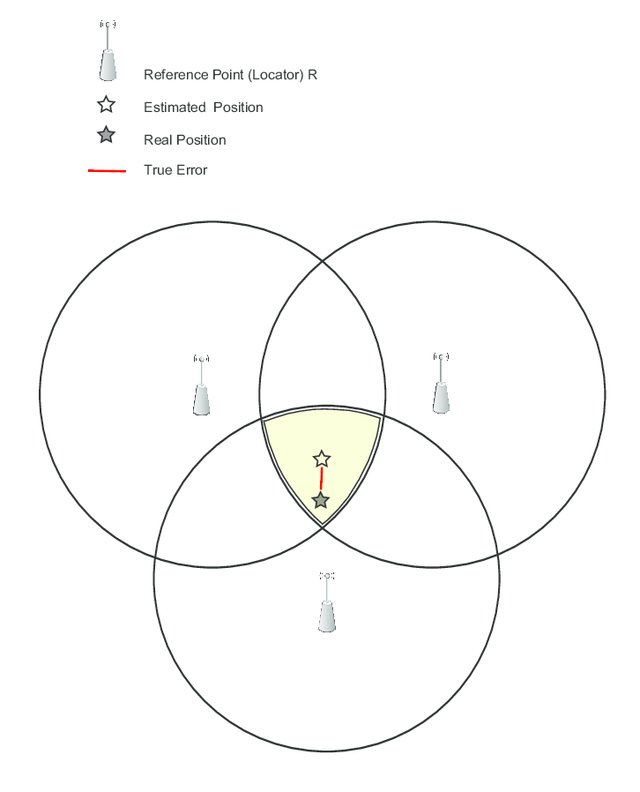
\includegraphics[scale=1]{./images/trilat}
    \caption{Algoritmo de Triangulación}
    \label{fig:Triangulación}
\end{figure}

\subsubsection{\textbf{Angulación}}
    \begin{enumerate}
        \item {\textbf{\ac{AoA}}: es una técnica que determina el ángulo de llegada de la señal, respecto de la ubicación conocida de estaciones base a través de envío de múltiples mensajes desde el Dispositivo móvil hacia el AP. Dado que la precisión de la medición del ángulo de llegada es la que permite estimar la posición, se tiene que estas deben ser altamente direccionales o bien, tratarse de un arreglo de antenas, lo que encarece el costo de sistemas que implementen este tipo de solución. Además, se tiene que esta técnica ve alteradas sus mediciones debido a efectos de la propagación multicamino de la señal cuando se trata de dispositivos que no se hallan en \ac{NLOS}.
        
        \begin{figure}[h!]
            \centering
            \begin{subfigure}[b]{0.3\textwidth}
               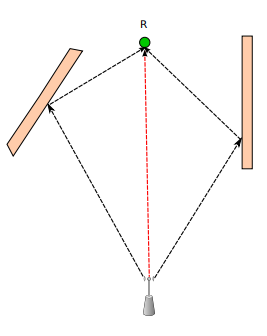
\includegraphics[width=\textwidth]{./images/los}
                \caption{Señal enviada en \ac{LOS}}
                \label{fig:LOS}
            \end{subfigure}
            \begin{subfigure}[b]{0.315\textwidth}
             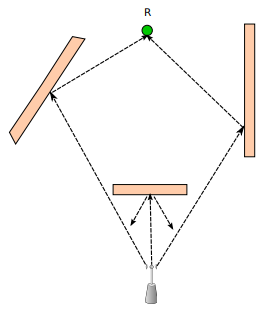
\includegraphics[width=\textwidth]{./images/nlos}
                \caption{Señal enviada en \ac{NLOS}}
                \label{fig:NLOS}
            \end{subfigure}
        \end{figure}
        
%%%%%%%%%%%%%%%%%%%%%%%%%%%%%%%%%%%%%%%%%%%%%%%%%%%%%%%%%%
                \clearpage 
%%%%%%%%%%%%%%%%%%%%%%%%%%%%%%%%%%%%%%%%%%%%%%%%%%%%%%%%%%

        
        Por esta razón, el sistema, aunque preciso en espacios exteriores, no es del todo idóneo para espacios interiores, ya que las reflexiones que se producen en paredes y otros objetos que cambian significativamente la dirección o ángulo de llegada de la señal y por tanto, degradan la precisión de la estimación de posición.
        
        \begin{figure}[h!]
            \centering
            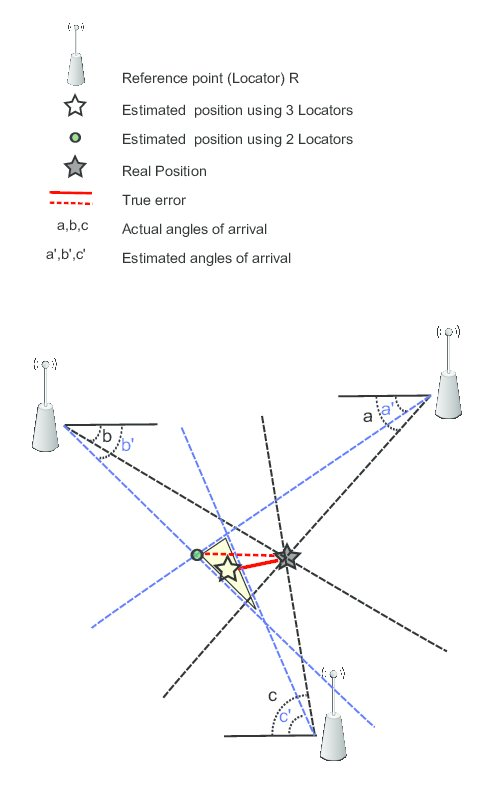
\includegraphics[scale=1.2]{./images/aoa}
            \caption{Técnica de Ángulo de Llegada (AoA)}
            \label{fig:AoA}
        \end{figure}
        }
    \end{enumerate}

%%%%%%%%%%%%%%%%%%%%%%%%%%%%%%%%%%%%%%%%%%%%%%%%%%%%%%%%%%
                \clearpage 
%%%%%%%%%%%%%%%%%%%%%%%%%%%%%%%%%%%%%%%%%%%%%%%%%%%%%%%%%%

\subsubsection{\textbf{Lateración}}

\begin{itemize}
    \item{\textbf{Técnicas basadas en la propagación por tiempo}
    
    \begin{enumerate}
        \item {\textbf{\ac{ToA}}: \label{ToA} El tiempo de llegada aparece como el tiempo de viaje del transmisor hasta el receptor y permite, si es que se le multiplica por la velocidad de la luz, obtener la distancia que separa ambos dispositivos. Para medir el tiempo de llegada en el aire, este método requiere sincronización previa de los dispositivos, que para hacer posicionamiento en el espacio, requiere de al menos 4 transmisores.\\
        
         \begin{figure}[h!]
            \centering
            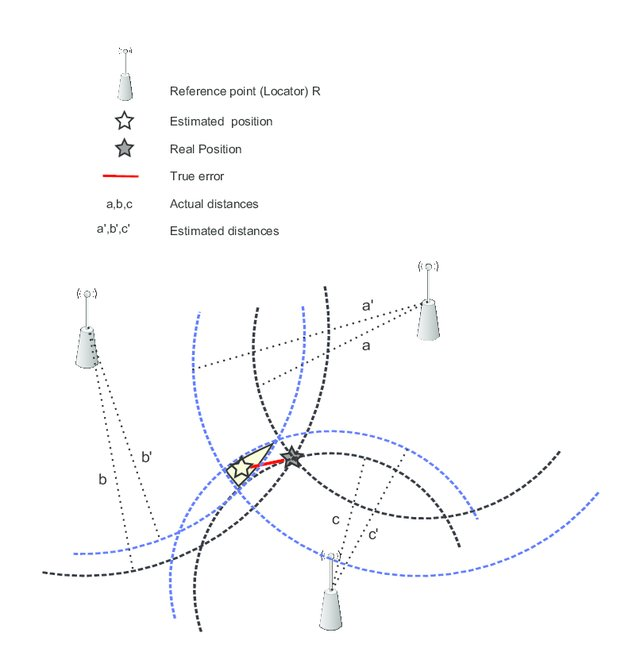
\includegraphics[scale=1]{./images/toa}
            \caption{Técnica de Tiempo de Llegada (ToA)}
            \label{fig:ToA}
        \end{figure}
            
        En ésta técnica, dado que los errores de estimación de distancia se derivan de mediciones de tiempo de salida y llegada del mensaje, se debe procurar que los tiempos sean bien medidos, esto es, que todos los dispositivos transmisor y receptor estén sincronizados en el mismo tiempo. La correcta implementación de un sistema de medición basado en ToA permite filtrar los efectos de la multitrayectoria.}\\
        
        \item {\textbf{\ac{TDoA}}: Esta técnica, acorde a lo mencionado en \cite{17}, cosiste en medir la diferencia de tiempo de llegada de la señal que se envia desde un objeto y que es recibida por otros tres dispositivos.\\
        
        Con TDoA, se puede iniciar la transmisión de la señal en un tiempo desconocido en tanto sea conocido por los otros nodos receptores. Lo único que se requiere para que esto funcione, es que entre los receptores, exista una sincronización de tiempo. Esta técnica, también conocida como Multilateración tiene como obstáculo el hecho de requerir una cantidad significativa de ancho de banda, así como también, el alto costo del equipamiento utilizado para aplicarlo.\\
        
        Y es que la banda usada para la implementación de esta tecnología es la \ac{UWB}, definido por la \ac{FCC} como la porción del espectro electromagnético con frecuencias que van desde los 3.1 hasta los 10.6 GHz.\\
        
            \begin{figure}[h!]
                \centering
                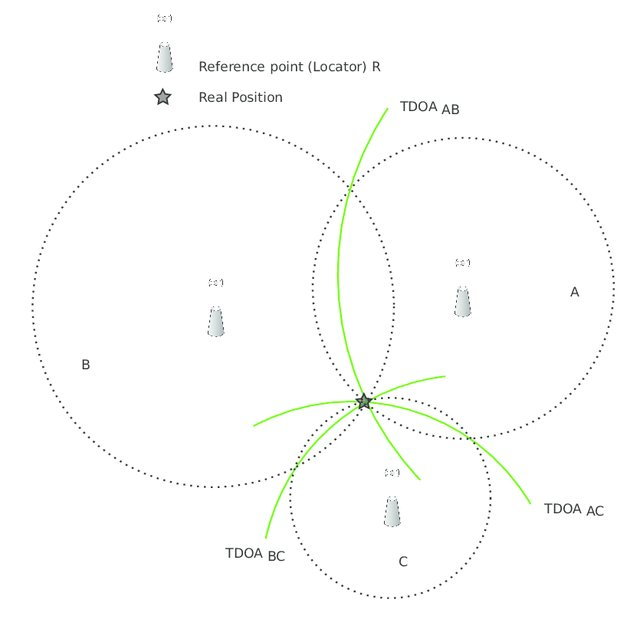
\includegraphics[scale=1]{./images/tdoa}
                \caption{Técnica de Diferencia de Tiempo de Llegada (TDoA)}
                \label{fig:TDoA}
            \end{figure}
        
        }
        \newpage 
        \item {\textbf{\ac{RToF}}: en este método basado en \ref{ToA} que consiste en el tiempo total que toma la conexión entre los dos dispositivos que participan en la comunicación. A diferencia de \ref{TDoA}, acá se considera el tiempo de ida y regreso de la señal, no sólo el tiempo que tarda desde el transmisor hasta el receptor. Este método de medida no requiere ninguna sincronización entre los dispositivos, de modo que se puede implementar necesitan únicamente enviar el resultado de la medición del \ac{RTT} para hacer el cálculo bajo la siguiente fórmula:\\
        
        \begin{equation}
            d = \dfrac{c\cdot{\left(T_{Total} - T_{proc}\right)}}{2}
        \end{equation}
        
        Donde \textit{d}, representa la distancia entre los dos dispositivos; \textit{c}, la velocidad de la luz; Tproc, el tiempo que le toma a la estación realizar el calculo. Siendo este último, un parámetro complejo de obtener con precisión, ya que depende de la latencia del sistema. Esto se escala como la principal desventaja de este sistema ya que calcular la posición para varios dispositivos se traduce en lidiar con latencias que impidan obtener la posición de dispositivos que se mueven rápidamente.\\
        
        \begin{figure}[h!]
            \centering
            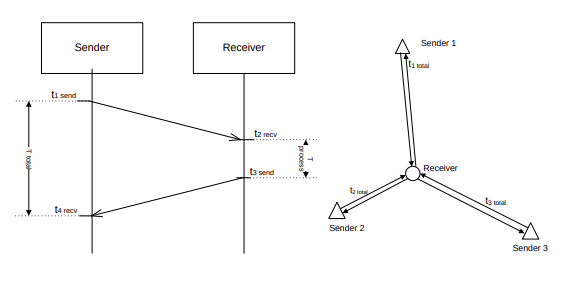
\includegraphics[scale=0.52]{Tesis/images/rtof}
            \caption{Diagrama de medición de distancia usando \ac{RToF}}
            \label{fig:RTOF}
        \end{figure}
        }
    \end{enumerate}
            }

    \item{\textbf{Técnicas basadas en los niveles de intensidad de señal recibida}
    \begin{enumerate}
        \item{\textbf{\ac{RSSI}}: Respecto de esta técnica se tiene que algunos autores la introducen como una técnica propia de algoritmos de Detección de Proximidad (\ref{Detección de Proximidad}}) debido a que los niveles de los indicadores de intensidad de señal recibida, al guardar relación con la distancia, tal y como señalan los modelos de propagación para interiores, establecen que a menor distancia del AP, mayor debe ser la intensidad de señal recibida.\\
        
        Los mismos autores que la clasifican dentro de la sección mencionada, utilizan esta técnica para trazar un sistema de coordenadas basadas en las intensidades recibidas respecto de cada AP, esto les permite mapear la zona en una etapa que llaman offline y ubicar al dispositivo en la etapa posterior, llamada online.\ \
            
        En esta etapa, se asigna a través de un sistema de coordenadas, los niveles de intensidad de señal, tal que es posible posicionar el objetivo según los RSS de los AP, como se ve en la imagen.
            
        \begin{figure}[h!]
            \centering
            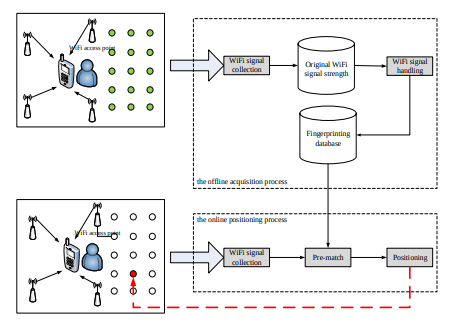
\includegraphics[scale = 0.6]{./images/rssi}
            \caption{Idea de algoritmo basado en RSSI}
            \label{fig:RSSI}
        \end{figure}
        
        \item{Algoritmos de posicionamiento para método por características de posición}\\
        
            \begin{enumerate}
                \item {\textbf{Método Probabilístico}: En este método, se considera el estimar la posición del ibjetivo, como un problema de clasificación, ya que desde un vector de RSS capturadas desde los APs, se puede estimar la probabilidad de que un valor \textit{S}, pertenezca a un AP particular, y por ende, a un punto de coordenadas aproximado. \\
                
                Se puede hacer el cálculo de la posición a través de modelos de inferencia y asociarlo también a un tipo de Cadenas de Markov, así como también, apoyar el cálculo introduciendo medidas de dispersión tales como la desviación estándar y la varianza, o de una medida de tendencia central como es la media.\\
                }
                
%%%%%%%%%%%%%%%%%%%%%%%%%%%%%%%%%%%%%%%%%%%%%%%%%%%%%%%%%%
                \clearpage 
%%%%%%%%%%%%%%%%%%%%%%%%%%%%%%%%%%%%%%%%%%%%%%%%%%%%%%%%%%
                
                \item{\textbf{Método \ac{SVM}}: \label{SVM} En la literatura consultada \cite{7} los autores señalan a esta técnica como \textit{''Una nueva u prometedora técnica para clasificación de datos y Machine Learning.''}, que ha sido usada con resultados satisfactorios en el mapeo de intensidad de señales inalámbricas.\\
                
                Su implementación consiste igualmente en dos fases; una de entrenamiento, que es aquella en que los sets con los datos de  intensidad de señal de los AP son ingresados, y con los cuales se buscará diseñar un hiperplano que clasifique los vectores en dos clases, procurando maximizar la distancia entre estos.\\
                
                \begin{figure}[h!]
                    \centering
                    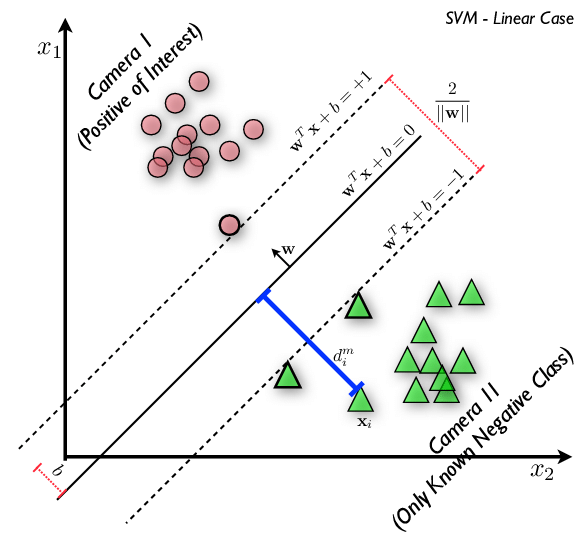
\includegraphics[scale=0.4]{./images/svm}
                    \caption{Distintos hiperplanos para el mismo set de datos.}
                    \label{fig:SVM}
                \end{figure}
                
                Sin embargo, dado que en un espacio indoor, la cantidad de AP es , por lo general, superior a 2, la posibilidad de que en un set de datos podamos diferenciar entre un AP u otro mediante el procedimiento de encontrar el hiperplano que separa maximizando la distancia entre los valores, es nula, e implementar un algoritmo recursivo que vaya evaluando para cada AP, el hiperplano que clasifica la medición del objetivo en alguno de ellos, es costosa computacionalmente además de compleja.\\
                }
%%%%%%%%%%%%%%%%%%%%%%%%%%%%%%%%%%%%%%%%%%%%%%%%%%%%%%%%%%
                \clearpage 
%%%%%%%%%%%%%%%%%%%%%%%%%%%%%%%%%%%%%%%%%%%%%%%%%%%%%%%%%%

                \item {\textbf{Método \ac{KNN}}: El método de vecinos más cercano es uno de los métodos de clasificación más simple dentro de la librería de Machine Learning ya que consiste, en una clasificación por similitud respecto de otros puntos en un dataset de entrenamiento. \\

                El objetivo de este método es el de agrupar vectores de características, que no son más que representaciones matemáticas para la información. Ha de tenerse en cuenta que el vector de características puede requerir un pre procesamiento si es que estas no son necesariamente numéricas, ya que de este modo se podrá agrupar los datos como si se tratara de un vector de $R^{N}$.\\

                Ahora, a diferencia de otros métodos de clasificación, como es el caso de \ref{SVM}, en KNN la fase de entrenamiento no existe, de manera que sólo se trata de una fase. En cambio, se tiene que cualquier caso por abstraer o generalizar la información que allí está, es un hecho en la etapa de clasificación.\\

                Esto significa que se puede trabajar inmediatamente sobre los datos, en tanto estos, tal y como se mencionó previamente, no requieran un pre procesamiento. Dado que lo que hace este método es agrupar valores, el resultado óptimo será cuando exista un reducido número de  data-sets y estos no tengan valores no numéricos.\\

                Así, se tiene que los datos que se clasificarán pueden también ser representados como una matriz de M x N  datos, de donde ; M, es el número de datos; y N, son las características de los datos. Dicho esto, el proceso de agrupamiento de los datos se hace según las siguientes consideraciones:\\

                \begin{itemize}
                    \item {Se calcularán las distancias entre los valores a clasificar, y aquellos contenidos en el data-set. En el cálculo de la distancia suele usarse la distancia euclidiana, que es básicamente, la magnitud del vector que se obtiene al restar un punto de muestra del data-set de entrenamiento, con el punto a clasificar
    
                    \begin{equation}
                        E(x,y) = \sqrt{\sum_{i=0}^{n}({x_{i}-y_{i}})^{2}} \ \ 
                    \end{equation}
                    }

                    \item{Se escogerá un valor \textit{K}, que por lo general, no es ni múltiplo de la cantidad de clases, ni par, y que representa la cantidad de valores \textit{K} con las distancias más bajas. Este puede ser escogido arbitrariamente o bien, en caso que sea necesario, obtenido por validación cruzada. \footnote{La validación cruzada o cross-validation es una técnica utilizada para evaluar los resultados de un análisis estadístico y garantizar que son independientes de la partición entre datos de entrenamiento y prueba.}\\}
                    
                    \item{Finalmente, se agruparán los datos a una clase, a través de la comparación de las distancias obtenidas. Si este, posee la mayoría de los  \textit{K} de puntos cuya distancia los asocia a una clase A, entonces este será clasificado en dicha clase. Si por el contrario, el número de puntos cuya distancia se acerca a los datos objetivo no son mayoría, entonces este pertenecerá a B.\\
                    
                    \begin{figure}[h!]
                        \centering
                        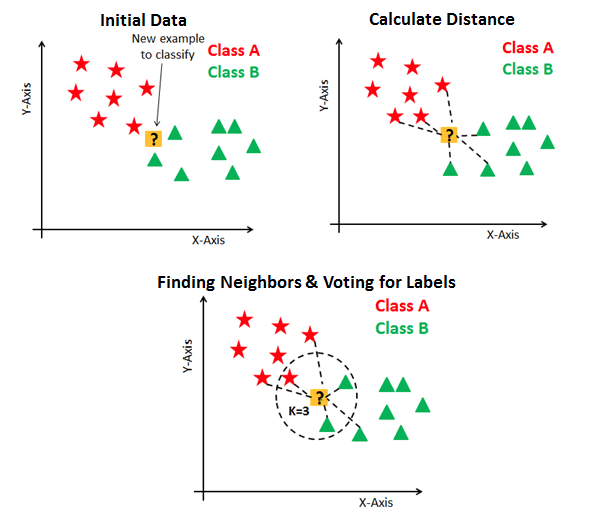
\includegraphics[scale=0.65]{./images/knn}
                        \caption{Representación gráfica del funcionamiento de \ac{KNN} según el valor de K}
                        \label{fig:KNN}
                    \end{figure}
                    }
            \end{itemize}}
            
            \newpage
            
            \item{\textbf{Método \ac{RN}}: Este método se vale de una neurona artificial llamada \textbf{perceptrón}, algo que fuera desarrollado entre los años 1950s y 1960s por el científico Frank Rosenblatt, inspirado por el trabajo de Warren McCulloch y Walter Pitts}<<A Logical Calculus of the Ideas Immanent in Nervous Activity>> \cite{19} donde señalan la posibilidad de rescatar la idea de un sistema complejo de redes y conexiones, de impulsos y señales, como es nuestro sistema nervioso, y extrapolarlo a uno computarizado, donde en lugar de estímulos, se tuvieran señales.
            
             Se mencionó que uno de los objetivos del trabajo de McCulloch fue el de introducir la noción de neurona artificial, por esto es que el perceptrón le debe su estructura, presentada a continuación: 
             
            \begin{figure}[h!]
                \centering
                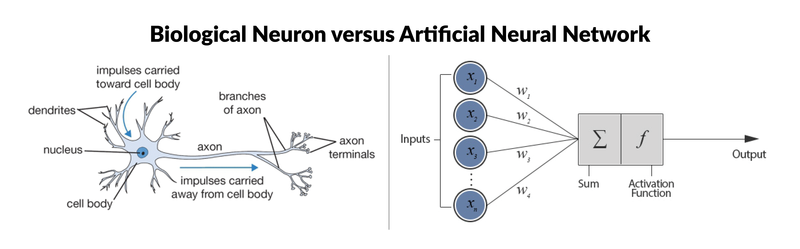
\includegraphics[scale=0.5]{Tesis/images/nn}
                \caption{Comparación por similitud de una neurona con un perceptrón}
                \label{fig:NN}
            \end{figure}
            
            En el cerebro humano, existen distintos tipos de neuronas las cuales están destinadas para tareas específicas, por esta razón, puede darse que una neurona reciba señales de temperatura, presión, luz, entre otras, antes de transmitir un impulso. Este último viene en algunos casos a ser la suma ponderada de los distintos estímulos nerviosos que provienen de las otras terminaciones sinápticas, tal que es en el soma donde se evalúa si esta excede el potencial de acción o no. Si lo hace, la señal será enviada a través del soma y las terminaciones sinápticas hasta un órgano diana u otra neurona, pudiendo ser esta señal inhibitoria, excitadora o moduladora.\\
            
            \begin{figure}
                \centering
                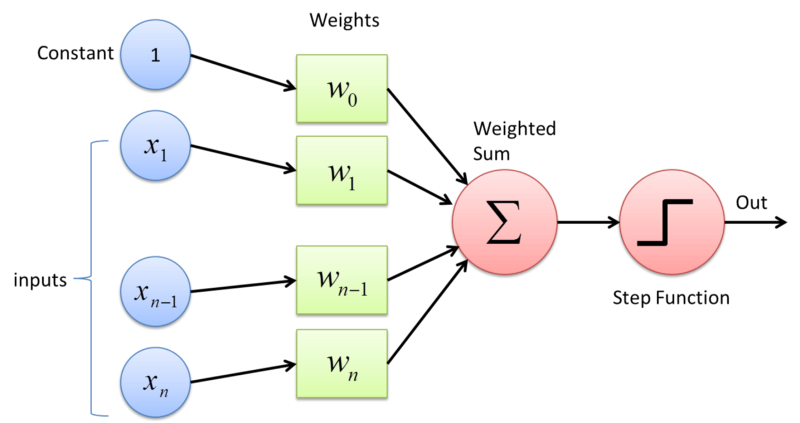
\includegraphics[scale=0.35]{Tesis/images/perceptron}
                \caption{Representación de un Perceptrón}
                \label{fig:Perceptron}
            \end{figure}
            
            Tal como se puede ver en \ref{fig:Perceptron}, se tiene que están las conexiones de la capa de entrada, representadas por impulsos o señales de entrada \textbf{$x_j$}, que luego se multiplican por los pesos \textit{$w_j$} y pasan a evaluarse en la función de activación.\\
            
            Las neuronas son representadas como unidades individuales de procesamiento, que al agruparse forman una red neuronal cuya función de activación, y luego, las capas se resumen en tres:\\
            
            \begin{itemize}
                \item {\textbf{Capa de entrada}: las unidades que componen esta capa son los campos de entrada, por donde ingresan los primeros estímulos}
                
                \item{\textbf{Conexiones ponderadas}: Las operaciones que se realizan en las capas, se logran a través de las fuerzas de conexión variables, o ponderaciones, que resultan del producto entre los pesos \textbf{$w_j$}, que representan la fuerza que tiene un nodo en particular, y los estímulos \textbf{$x_j$}. Los datos de entrada se presentan en la primera capa y estos se propagan a través de las capas ocultas, en forma de \textit{función de propagación},tal cual hiciera el impulso eléctrico en las neuronas, hasta llegar a la capa de salida que es donde el dato de salida, nos permitirá tomar decisiones o evaluar resultados.}
                
                \item{\textbf{Capas Ocultas}:  Son aquellas unidades de procesamiento que transforman el impulso de entrada en otro diferente pero que no son realmente ni una entrada ni una salida.}
                
                \item{\textbf{Función de activación}: Es quizás la característica principal o definitoria de las neuronas, la que mejor define el comportamiento de la misma. Se usan diferentes tipos de funciones, desde simples funciones simples de umbral a funciones no lineales. Se encarga de calcular el nivel o estado de activación de la neurona en función de la entrada total.\\
                
                La función de activación, en este caso Sigmoide, corresponde una función continua no lineal cuyo rango va entre 0 y 1 que puede ser representada gráficamente a través de \ref{fig:sigmoid} y matemáticamente a través de \ref{sigmoid_eq}:\\
            
                \begin{figure}[h!]
                    \centering
                    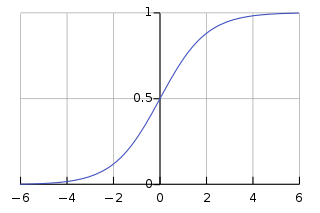
\includegraphics[scale=0.6]{./images/sigmoid}
                    \caption{Función Continua no lineal Sigmoide}
                    \label{fig:sigmoid}
                \end{figure}
            
                \begin{equation}
                    S(u_j) = \dfrac{1}{1+e^{-u_j}}
                    \label{sigmoid_eq}
                \end{equation}
                }       
                
                \item{\textbf{Capa de salida}: Compuesta por una o varias unidades que representan los campos de salida y que entregan el resultado que finalmente es modelado por la siguiente expresión:\\
                
                \begin{equation}
                    O_j  = S({w_j}{x_j} + {w_0})
                    \label{prob_pred}
                \end{equation}
                
                Donde $w_0$, es el  Bias, una constante que ayuda al modelo de una manera que puede ajustarse mejor a los datos dados y $O_j$, el resultado particular de la evaluación de un dato en la función Sigmoide.\\
                }
            \end{itemize}
            
            Al igual que hace el cerebro por acción de las neuronas, una red es capaz de aprender examinando los registros individuales, generando una predicción para cada uno de estos y ajustando, a través de los pesos, las ponderaciones en caso que el resultado no haya sido el óptimo. Este proceso es iterativo y puede tener lugar cientos de veces antes que la red sea capaz de mejorar sus predicciones antes de alcanzar resultados que satisfagan los criterios de parada.\\
            
            En un comienzo, las ponderaciones son aleatorias, y las respuestas suelen ser muy dispares, sin embargo, y conforme va avanzando el entrenamiento, esta va mejorando, haciéndose más precisa en predecir o replicar a partir de los resultados conocidos.\\
            
            Un aspecto importante, es que a la propagación de las respuestas desde las capas de entrada hacia la capa de salida, se le llama \textit{forward propagation} o \textit{propagación hacia adelante} y cuyo objetivo, así como el del entrenamiento en general es minimizar el costo computacional de la red. Ahora, así como existe la propagación hacia adelante, existe también una hacia atrás llamada \textit{back propagation}, que consiste en reingresar al sistema, la salida resultante de proceso anterior, a fin de optimizar el resultado de los pesos y sesgos. 
            \end{enumerate}
        \end{enumerate}
            }
    \end{itemize}
    
%	\chapter{Conclusiones}

% ***********************************************************************************
\section{Sumario}
Dentro del desarrollo del estudio, se contemplaron diversos enfoques, se ponderó la posiblidad de implementar en la memoria de título un sistema de posicionamiento indoor basándose en algoritmos de estimación de posición geométricos y otros, en parámetros más complejos, no obstante, la poca practicidad y adaptabilidad de estos modelos al ambiente donde se podría implementar, supone una desventaja innegable.

% ***********************************************************************************
\section{Conclusiones}
Por todo lo revisado, estudiado y expuesto, se plantea la posibilidad de que, como alternativa a los algoritmos geométricos o basados en potencia, se consideren alternativas más efectivas, de menor coste computacional y que no dependan de parámetros relacionados con el ambiente, dado que en ambientes indoor o en sectores muy concurridos hay métricas que varían considerablemente, al punto de obligar a realizar mediciones correctivas.\\

Además, se tiene que la efectividad y precisión del método que recoge las solicitudes IRDP, es considerablemente superior al no depender de otros parámetros salvo la llegada de los paquetes al router.\\

Se dio cumplimiento a los objetivos planteados inicialmente, mediante la investigación de las alternativas, que fueron abordadas a fondo a través de literatura. Se pudo llegar a una comprensión justificada de las ventajas y desventajas de los métodos, pudiendo así, escoger con base en distintos estudios teóricos y empíricos, cuál es el método que convendría desarrollar en detalle en la memoria de título.\\

En suma, se destaca la importancia de llegar a desarrollar un sistema de posicionamiento indoor que cuente con una precisión que no sea directamente proporcional a la capacidad de cómputo, tanto si se desea resolver necesidades humanas tales como, hallar la mejor ruta de acceso para una persona con capacidades diferentes, a través de una aplicación móvil que desde el seguimiento de su interfaz vaya dándole instrucciones. Como si se desea implementar un sistema que recoja las solicitudes de los clientes que desean conectarse y con ello, hacer un seguimiento de las posiciones, a fin de que este, permita generar reportes e informes estadísticos que relacionen patrones de conducta y también de consumo, que favorezcan a un mejoramiento en las estrategias de venta y en la experiencia de compra del cliente.

% ***********************************************************************************
\section{Trabajo Futuro}
Se listan las posibles líneas de investigación que se deducen directamente de la presente obra.

\begin{enumerate}
\item {Implementación de un sistema que realice el seguimiento de las solicitudes IRDP donde pueda visualizarse el movimiento de las interfaces de red}
\item{Realizar un estudio que contraste la precisión y eficacia con la que los métodos geométricos y el de las solicitudes IRDP realizan la estimación de posición.}
\item{Estudiar algoritmos de posicionamiento basado en redes neuronales.}
\item{Estudiar la precisión de las mediciones obtenidas por el uso del sistema presentado en \cite{8}}
\end{enumerate}

Se quiere que al menos existan unas 3 a 5 ideas en las que se pueda seguir investigando.

% ***********************************************************************************
%\section{Publicación}
%A veces, los trabajos dan pie a una publicación en conferencia o revista. Es importante mencionarlo en esta sección.


% ******************** Bibliografía ********************
\pdfbookmark{Bibliografía}{bibliografia}
%\chapter{Bibliografía}

\begin{thebibliography}{X}
\bibitem{1} \textsc{Van Vinh Nguyen} y \textsc{Weon Lee Jong}, <<Self-Positioning System for Indoor Navigation on Mobile Phones>> \textit{IEEE International Conference on Consumer Electronics (ICCE), 2012}

\bibitem{2} \textsc{Rea Mauricio, Cordobés Héctor, Gustiniano Domenico},<<Twins: Time-of-flight based Wireless Indor Navigation System>>

\bibitem{3} \textsc{Bianca Bobescu, Marian Alexandru} <<Mobile indoor positioning using Wifi localization>> Review of the Air Force Academy. Transilvania University, Brasov, Romania

\bibitem{4} \textsc{Mayur Tawari},\textsc{Onkar Pathak},\textsc{Rajesh Palaskar} y \textsc{Rajesh Palkar}, <<Wi-Fi Indoor Positioning System Based on RSSI Measurements from Wi-Fi Access Points –A Tri-lateration Approach>>, \textit{International Journal of Scientific \& Engineering Research. V5}, 2014.

\bibitem{5} \textsc{C. Yang and H. r. Shao}, <<WiFi-based indoor positioning,>> in IEEE Communications Magazine, vol. 53, no. 3, pp. 150-157, March 2015. doi: 10.1109/MCOM.2015.7060497

\bibitem{6} \textsc{Zahid Farid, Rosdiadee Nordin} y \textsc{Mahamod Ismail}, <<Recent Advances in Wireless Indoor Localization Techniques and System>>, \textit{Journal of Computer Networks and Communications}, 2013.

\bibitem{7} \textsc{Zhao Kai, Li Binghao} y \textsc{Andrew Dempster}, <<A Comparison of algorithms adopted in fingerprinting indoor positioning systems>>, \textit{IGNSS Symposium}, 2013.

\bibitem{8} \textsc{Ma, R., Guo, Q., Hu, C., \& Xue, J.} (2015). <<An Improved WiFi Indoor Positioning Algorithm by Weighted Fusion>>. Sensors.

\bibitem{9} \textsc{Habibi Lashkari, Arash \& Parhizkar, Behrang \& Ng Ah Ngan, Mike.} (2010). <<WIFI-based indoor positioning system>>. Computer and Network Technology, International Conference on. 76-78. 10.1109/ICCNT.2010.33. 

\bibitem{10} \textsc{Zourmand A., Sheng N., Lai Kun A., et al},<<Human Counting and Indoor Positioning System Using WiFi Technology>> , \textit{IEEE, International Conference on Automatic Control and Intelligent Systems.} October 20,2018, Shah Alam, Malaysia.

\bibitem{11} \textsc{Davies K., Jones I.} y \textsc{Shapiro J.},<<A Bayesian Approach to Dealing with Device Heterogeneity in an Indoor Positining System , \textit{International Conference on Indoor Positioning and Indoor Navigation.} September 2018, Nantes, France.

\bibitem{12} \textsc{Le Dortz N, Zetterberg P. & Gain F.}, <<Wifi Fingerpirnt Indoor Positioning System Using Probability Distribution Comparison>>, \textit{IEEE ICASSP 2012}
\bibitem{13} \textsc{Beom-Ju Shin, Kwang-Won Lee, Sun-Ho Choi, et al},<<Indoor WiFi positining System fior Android Based Smartphone>> , \textit{ICTC 2010}

\bibitem{14} \textsc{Lu Y., Zhang D. Cheng Y., et al},<<An Improved Method and Implementation of Indoor Positioning Fingerprint Matching Localization Based on WLAN>>, \textit{Springer Nature},Switzerland AG 2019

\bibitem{15} \textsc{},<<Towards the Implementation of Recurrent Neural Networks Schemes for WiFi Fingerprint-Based Indoor Positioning>> , \textit{IEEE 2018}

\bibitem{16} \textsc{Y Lu et al},<<Implementation of Fingerprint Matching Method for Indoor Position Based on Virtual Reality Technology>>
\end{thebibliography}

\begin{thebibliography}{X}
\bibitem{1} \textsc{Van Vinh Nguyen} y \textsc{Weon Lee Jong}, <<Self-Positioning System for Indoor Navigation on Mobile Phones>> \textit{IEEE International Conference on Consumer Electronics (ICCE), 2012}
\bibitem{2} \textsc{Rea Mauricio, Cordobés Héctor, Gustiniano Domenico},<<Twins: Time-of-flight based Wireless Indor Navigation System>>
\bibitem{3} \textsc{Bianca Bobescu, Marian Alexandru} <<Mobile indoor positioning using Wifi localization>> Review of the Air Force Academy. Transilvania University, Brasov, Romania
\bibitem{4} \textsc{Mayur Tawari},\textsc{Onkar Pathak},\textsc{Rajesh Palaskar} y \textsc{Rajesh Palkar}, <<Wi-Fi Indoor Positioning System Based on RSSI Measurements from Wi-Fi Access Points –A Tri-lateration Approach>>, \textit{International Journal of Scientific \& Engineering Research. V5}, 2014.
\bibitem{5} \textsc{C. Yang and H. r. Shao}, <<WiFi-based indoor positioning,>> in IEEE Communications Magazine, vol. 53, no. 3, pp. 150-157, March 2015. doi: 10.1109/MCOM.2015.7060497
\bibitem{6} \textsc{Zahid Farid, Rosdiadee Nordin} y \textsc{Mahamod Ismail}, <<Recent Advances in Wireless Indoor Localization Techniques and System>>, \textit{Journal of Computer Networks and Communications}, 2013.
\bibitem{7} \textsc{Zhao Kai, Li Binghao} y \textsc{Andrew Dempster}, <<A Comparison of algorithms adopted in fingerprinting indoor positioning systems>>, \textit{IGNSS Symposium}, 2013.
\bibitem{8} \textsc{Ma, R., Guo, Q., Hu, C., \& Xue, J.} (2015). <<An Improved WiFi Indoor Positioning Algorithm by Weighted Fusion>>. Sensors.
\bibitem{9} \textsc{Habibi Lashkari, Arash \& Parhizkar, Behrang \& Ng Ah Ngan, Mike.} (2010). <<WIFI-based indoor positioning system>>. Computer and Network Technology, International Conference on. 76-78. 10.1109/ICCNT.2010.33. 
\bibitem{10} \textsc{Zourmand A., Sheng N., Lai Kun A., et al},<<Human Counting and Indoor Positioning System Using WiFi Technology>> , \textit{IEEE, International Conference on Automatic Control and Intelligent Systems.} October 20,2018, Shah Alam, Malaysia.
\bibitem{11} \textsc{Davies K., Jones I.} y \textsc{Shapiro J.},<<A Bayesian Approach to Dealing with Device Heterogeneity in an Indoor Positining System>>, \textit{International Conference on Indoor Positioning and Indoor Navigation.} September 2018, Nantes, France.

\bibitem{12} \textsc{Le Dortz N, Zetterberg P. and Gain F.}, <<Wifi Fingerpirnt Indoor Positioning System Using Probability Distribution Comparison>>, \textit{IEEE ICASSP 2012}
\bibitem{13} \textsc{Beom-Ju Shin, Kwang-Won Lee, Sun-Ho Choi, et al},<<Indoor WiFi positining System fior Android Based Smartphone>> , \textit{ICTC 2010}
\bibitem{14} \textsc{Lu Y., Zhang D. Cheng Y., et al},<<An Improved Method and Implementation of Indoor Positioning Fingerprint Matching Localization Based on WLAN>>, \textit{Springer Nature},Switzerland AG 2019
\bibitem{15} \textsc{},<<Towards the Implementation of Recurrent Neural Networks Schemes for WiFi Fingerprint-Based Indoor Positioning>> , \textit{IEEE 2018}
\bibitem{16} \textsc{Y Lu et al},<<Implementation of Fingerprint Matching Method for Indoor Position Based on Virtual Reality Technology>>, \textit{An Improved Method and Implementation}
\end{thebibliography}

% ******************** Anexos ********************
	\appendix
%	\chapter{Códigos}

%*******************************************************************************%
\section{Derivación de fórmulas}

Lorem ipsum dolor sit amet, consectetur adipiscing elit, sed do eiusmod tempor incididunt ut labore et dolore magna aliqua. Ut enim ad minim veniam, quis nostrud exercitation ullamco laboris nisi ut aliquip ex ea commodo consequat.


%*******************************************************************************%
\section{Unidades especiales}

Lorem ipsum dolor sit amet, consectetur adipiscing elit, sed do eiusmod tempor incididunt ut labore et dolore magna aliqua. Ut enim ad minim veniam, quis nostrud exercitation ullamco laboris nisi ut aliquip ex ea commodo consequat.

	
\end{document}